% !TEX TS-program = pdflatex
% !TEX encoding = UTF-8 Unicode

% This is a simple template for a LaTeX document using the "article" class.
% See "book", "report", "letter" for other types of document.

\documentclass[11pt]{report} % use larger type; default would be 10pt

\usepackage[utf8]{inputenc} % set input encoding (not needed with XeLaTeX)

%%% Examples of Article customizations
% These packages are optional, depending whether you want the features they provide.
% See the LaTeX Companion or other references for full information.

%%% PAGE DIMENSIONS
\usepackage{geometry} % to change the page dimensions
\geometry{a4paper} % or letterpaper (US) or a5paper or....
\geometry{margin=1.5in} % for example, change the margins to 2 inches all round
% \geometry{landscape} % set up the page for landscape
%   read geometry.pdf for detailed page layout information

\usepackage{graphicx} % support the \includegraphics command and options
\graphicspath{{Figures/}} % Set the default folder for images

% \usepackage[parfill]{parskip} % Activate to begin paragraphs with an empty line rather than an indent

%%% PACKAGES
\usepackage{booktabs} % for much better looking tables
\usepackage{array} % for better arrays (eg matrices) in maths
\usepackage{paralist} % very flexible & customisable lists (eg. enumerate/itemize, etc.)
\usepackage{verbatim} % adds environment for commenting out blocks of text & for better verbatim
\usepackage{subfigure} % make it possible to include more than one captioned figure/table in a single float
\usepackage{cleveref}  % For referencing more than one equation at at time
\usepackage[colorlinks=true,urlcolor=blue,citecolor=blue,linkcolor=black]{hyperref} % for hyper referencing
\usepackage{amsmath}
\usepackage[numbers,sort&compress]{natbib}  % Make a group of citations appear in order in the document
% These packages are all incorporated in the memoir class to one degree or another...

%%% HEADERS & FOOTERS
\usepackage{fancyhdr} % This should be set AFTER setting up the page geometry
\pagestyle{fancy} % options: empty , plain , fancy
\renewcommand{\headrulewidth}{0pt} % customise the layout...
\lhead{}\chead{}\rhead{}
\lfoot{}\cfoot{\thepage}\rfoot{}

%%% SECTION TITLE APPEARANCE
\usepackage{sectsty}
\allsectionsfont{\sffamily\mdseries\upshape} % (See the fntguide.pdf for font help)
% (This matches ConTeXt defaults)

% New commands
\newcommand\numberthis{\addtocounter{equation}{1}\tag{\theequation}}  % For numbering only one equation in an array.

%%% ToC (table of contents) APPEARANCE
\usepackage[nottoc,notlof,notlot]{tocbibind} % Put the bibliography in the ToC
\usepackage[titles,subfigure]{tocloft} % Alter the style of the Table of Contents
\renewcommand{\cftsecfont}{\rmfamily\mdseries\upshape}
\renewcommand{\cftsecpagefont}{\rmfamily\mdseries\upshape} % No bold!

%%% END Article customizations

%%% The "real" document content comes below...
% \title{Brownian motors thermally coupled to the environment}
% \author{Jack Devine}
%\date{} % Activate to display a given date or no date (if empty),
         % otherwise the current date is printed

\begin{document}
	\begin{titlepage}
		\centering
		{\huge\bfseries Self induced temperature gradients in Brownian dynamics\par}
		\vspace{1cm}
		{\huge Jack Devine\par}
		\vspace{1cm}
		{\scshape\LARGE The University of Otago \par}
		\vspace{1cm}
		\includegraphics[width=0.45\textwidth]{ou-logo.png}\par\vspace{1cm}
		\vspace{1cm}
		{\scshape\Large A thesis submitted for Honours in physics at the University of Otago, Dunedin, New Zealand\par}
		\vspace{1.5cm}
		\vspace{2cm}
		\vfill
		supervised by\par
		Dr M. W. \textsc{Jack}

		\vfill

	% Bottom of the page
		{\large \today\par}
	\end{titlepage}


\newpage

%----------------------------------------------------------------------------------------
%	ABSTRACT
%----------------------------------------------------------------------------------------
%
\begin{center}
\section*{Abstract} % This section will not appear in the table of contents due to the star (\section*)
\end{center}

Brownian motors are capable of converting chemical energy directly into work and are crucial for many biological processes. The purpose of this project is to consider the motors thermal interaction with  the environment, we want to know whether these thermal interactions will change the properties of the Brownian motors as compared to calculations made without considering coupling to the environment.

%----------------------------------------------------------------------------------------

\newpage % Start the article content on the second page, remove this if you have a longer abstract that goes onto the second page

\tableofcontents

%----------------------------------------------------------------------------------------
%	INTRODUCTION
%----------------------------------------------------------------------------------------

\chapter{Introduction}

Brownian motors are devices that can use stored energy to create directed motion on a microscopic scale. As well as being able to crank a rotor in the in the fashion of a traditional motor, they are also able to pump ions against a gradient and translocate molecules. Brownian motors have been implemented in the laboratory, for example Ref \cite{BlickleBechinger2011} created a stochastic heat engine by placing a single colloidal particle in a time dependent optical trap. Likewise, Ref \cite{Pedro2014} placed a colloidal particle in an optical tweezer and drove the particle with explosive vaporization of the surrounding liquid, thus demonstrating a thermal mechanism for Brownian motors. Brownian motors also include devices that can transport molecules over a long distance, for example Ref \cite{JoelBader1999} placed DNA molecules in a time dependent potential to transport the molecules. A very important class of Brownian motors are those where the energy is supplied by a chemical reaction. None of the above experiments fit this criteria, however these types of motors are ubiquitous in biology \cite{PhillipsQuakeMay2006, Magnasco1994}. Recently, thanks to improvements in imaging techniques, researchers have been able to make highly detailed images of these motors and their working components \cite{YiWeiChang2016}.

In this project, we will model Brownian motors using concepts from statistical mechanics. In particular, a Brownian motor will be modeled by a Brownian particle diffusing over its free energy landscape \cite{Reimann2001}, which in one dimension will be denoted by $x$. In the case of Brownian motion, it is natural to think of $x$ as a spatial coordinate, however in the case of Brownian motors this is not always the case. Often we will think of $x$ as a reaction coordinate for a chemical reaction, or in the case of a rotary motor, it could be the angle of the motor. We will think of a Brownian particle moving in titled periodic potential of the form $V(x) = f x + v_0(x)$ for some external forcing $f$ and some periodic function $v_0(x)$ with period $L$. This is shown schematically in figure \ref{fig:Schematic}, in this figure we have a particle with a certain known probability density. The particle is agitated by thermal vibrations in a random diffusive manner, however there is also a forcing on the particles that we describe using the potential. Different types of Brownian motors have been explored in the literature, including the Feynman ratchet \cite{Feynman1963}, the Landauer blowtorch \cite{Landauer1988}, thermal ratchets \cite{Pedro2014}, time dependent potentials \cite{JoelBader1999,BlickleBechinger2011} and tilted periodic potentials \cite{Leibler1993,Magnasco1994}.

\begin{figure}[tb]
	\centering
	\subfigure{%
		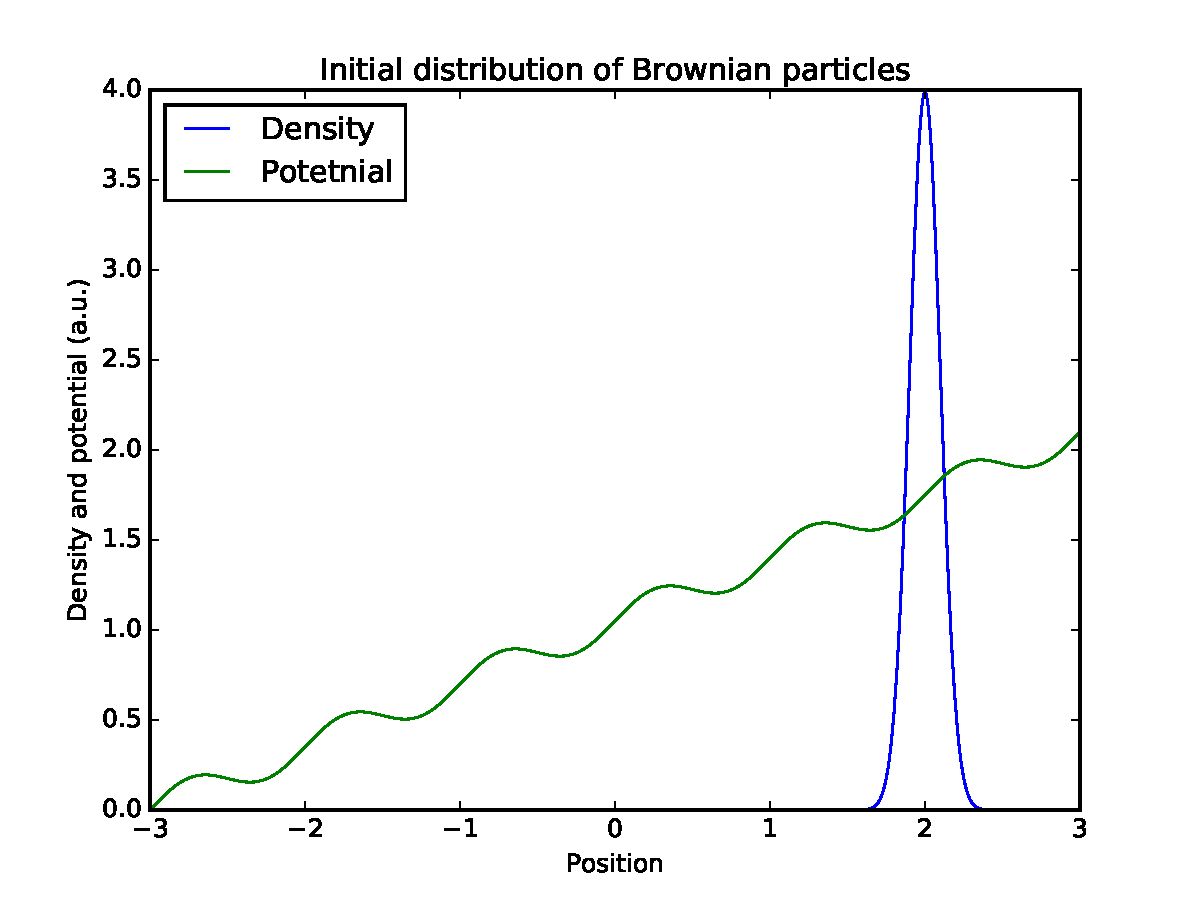
\includegraphics[width=0.45\columnwidth]{SchematicConstantTempInit}
	}
\quad
	\subfigure{
		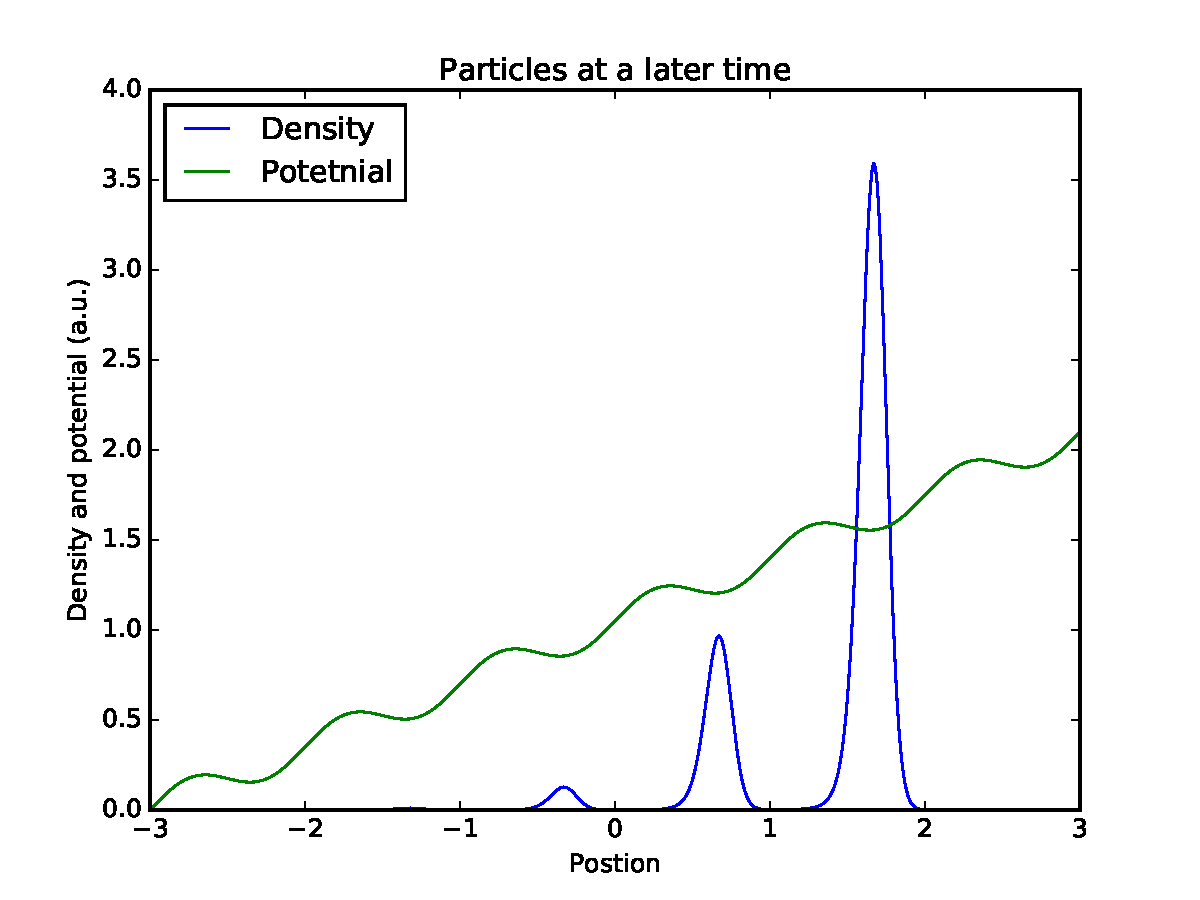
\includegraphics[width=0.45\columnwidth]{SchematicConstantTempFinal}
	}
\caption{Schematic showing the probability density of particles diffusing in a one dimensional periodic potential at a fixed temperature. We see that the particles tend to drift down the potential as they diffuse, this drift will be called the current $J$ which we will quantify in section \ref{Smoluchowski}.}
\label{fig:Schematic}
\end{figure}

\section{Classes of Brownian motors} \label{BrownianMotorClasses}
Here we will discuss different classes of Brownian motors and their relationship to this project.

\subsection{Feynman ratchet and pawl}
The Feynman ratchet was initially discussed in the Feynman lectures \cite{Feynman1963} and was at first thought to be able to achieve greater than Carnot efficiency, however closer analysis showed that this was not possible \cite{ParrondoEspanol1996}. The system works as follows, we have two boxes that are thermally insulated from one another that are connected by an axle that can rotate. In one box there is a ratchet and pawl connected to the axle that makes it easy for the axle to turn one way (say clockwise), but hard to turn the other way (anti-clockwise). In the other box the axle is connected to paddles that are being buffeted by a gas (which we call the bath). The motion of the paddles are random since they are dictated by Brownian motion, so the purpose of the ratchet and pawl is to rectify the Brownian motion of these paddles. One may think that this could be used to do work (for example by using the axle to lift a weight), however this is not true. The problem is that the ratchet and pawl themselves will also be subject to random motion so they will sometimes allow the axle to turn anti-clockwise. To model the Feynman ratchet, we will need two degrees of freedom \cite{M.W.Jack2016}, this is beyond the scope of this project because we will only simulate systems with one degree of freedom.

\subsection{Landauer blowtorch}
The Landauer blowtorch scheme involves a temperature that varies in space \cite{Landauer1988}. As noted earlier, in order for the particles in Figure \ref{fig:Schematic} to get out of potential wells, they will need to acquire thermal energy from the environment. Landauer's idea was to assist these particles by heating the environment at the hills that the particles need to climb. From this Landauer notes that \cite{Landauer1988} ``The relative occupation of competing states of local stability is not determined solely by the characteristics of the locally favored states, but depends on the noise along the whole path connecting the competing states." This means that when we are modeling our system, we need to take non-constant temperatures into account.

\subsection{Thermal ratchet}
\cite{Pedro2014}

\subsection{Time dependent potentials}

\begin{figure}[tb]
	\centering
	\subfigure{%
		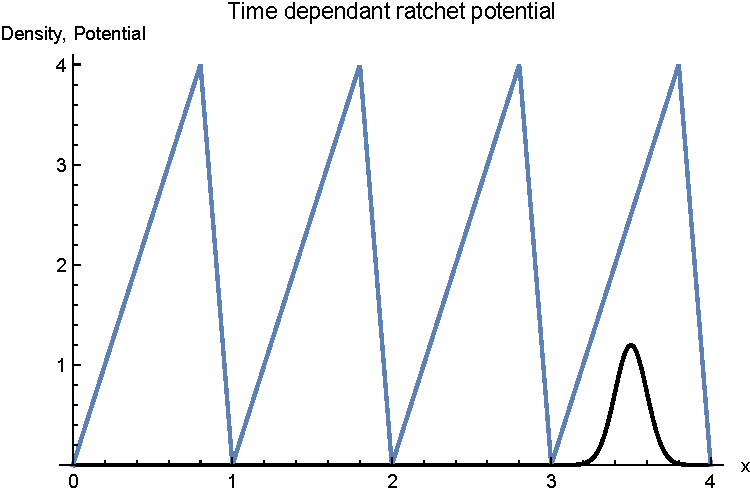
\includegraphics[width=0.45\columnwidth]{TimeDependentInit}
	}
\quad
	\subfigure{
		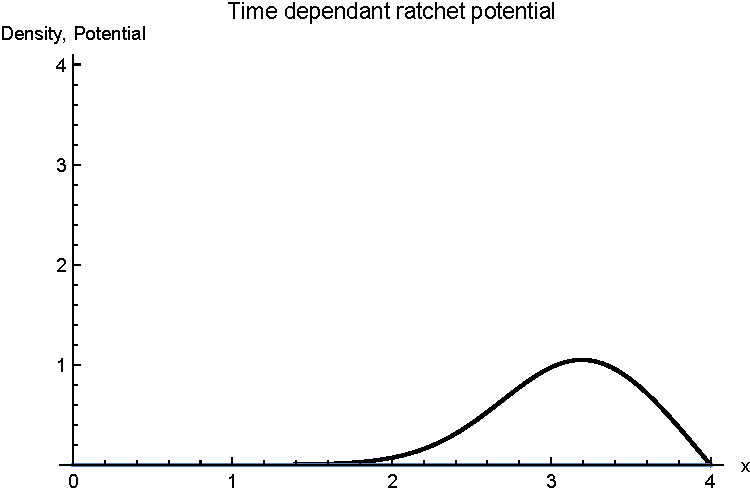
\includegraphics[width=0.45\columnwidth]{TimeDependentLater}
	}
	\subfigure{
		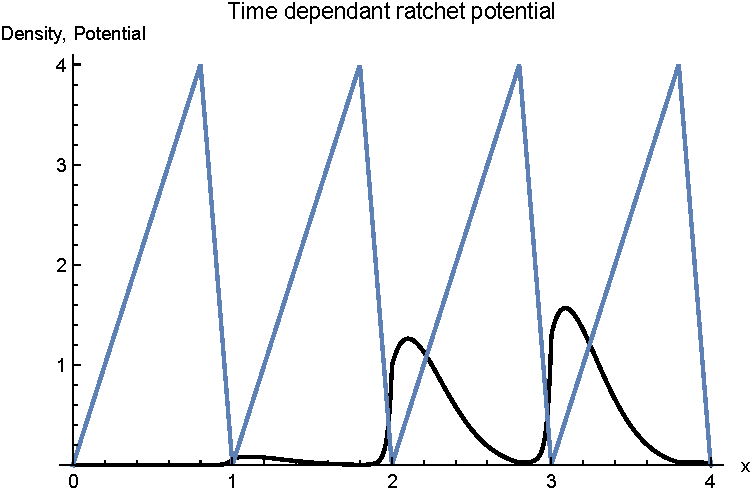
\includegraphics[width=0.45\columnwidth]{TimeDependentFinal}
	}
\caption{Schematic of particles diffusing in a time dependent potential, the blue line represents the potential and the black line represents the particle probability density. In (a) the particles are stuck in the first potential well, a certain time later the electric field is turned off and the particles diffuse freely as shown in part (b). When the potential is turned back on again, a large number of the particles will get stuck in the well to the left of the first one thus creating a net current to the left.}
\label{fig:TimeDependent}
\end{figure}

Both \cite{BlickleBechinger2011} \cite{JoelBader1999} are examples of experiments where a time dependent potential was used to do work on molecules. In \cite{JoelBader1999} DNA molecules are placed in a time dependent ratchet potential. When the electric field is on it creates a saw tooth shaped potential as shown in Figure \ref{fig:TimeDependent}, when the electric field is on, the molecules will go to the bottom of the wells and get stuck there. When the electric field is turned off however, the molecules will diffuse freely so that when the potential is turned back on at a later time, a large number of the molecules will then get trapped in the well to the left of where they were originally. Thus there is a net drift to the left.

\subsection{Tilted periodic potentials}
The tilted periodic potential (Figure \ref{fig:Schematic}) is of particular interest for this project because it can be used to model biological motors \cite{Leibler1993,Magnasco1994}. One way to model Brownian motors of this class is to think of a reaction coordinate $x$ that describes the conformation of a molecule in a chemical reaction. An example of this is the reaction ATP $\rightleftharpoons$ ADP + P, where ATP is adenosine tri-phosphate, ADP is adenosine di-phosphate and P is a lone phosphate molecule. This reaction coordinate is then coupled to a mechanical coordinate $y$ so that each time that a reaction takes place, the motor will move in some way. Since this is a chemical reaction, the free energy will be decreased as time moves forwards. So a system that has a potential that is periodic in $x$ is not sufficient to describe this situation, we will need to ``tilt" the potential by adding a forcing $f$. The value of $f$ will depend on the $\Delta G$ of the reaction (i.e. how far out of equilibrium the reaction is). It is shown in \cite{Magnasco1994} that this can be modeled by the two dimensional Smoluchowski equation. In this project we will only be modeling the one dimensional Somluchowski equation, so we will have to consider the case where $x$ and $y$ are tightly coupled. An example of tight coupling is the kinesin motor \cite{Leibler1993} that is used in cells to transport molecules. The kinesin motor is strongly bound to a track that it ``walks" along, on each step the motor will hydrolyze an ATP molecule using the reaction shown above. This reaction liberates about $12 k_B T$ Joules of energy that the motor uses to move forward. Kinesin motors are able to take many steps forward while taking few steps backwards all while falling off their track very infrequently \cite{BlockSM1990}.

\section{The Smoluchowski equation coupled interacting with the environment} \label{Smoluchowski}

As we will see, the diffusion is increased by increasing the temperature and the drift is increased by increasing $f$. In some cases such as the Landauer blowtorch, the environment has a non uniform temperature held fixed by an external heat source \cite{Landauer1988}. With this in mind, we interpret Figure \ref{fig:Schematic} as follows: Brownian particles are subject to a given potential and are agitated by thermal noise, these agitations can give the particles the energy to move over barriers created by the potential. As one could imagine, these thermal interactions draw energy from the environment causing the temperature of the environment to change. Normally two simplifying assumptions are made at this point \cite{Reimann2001}, (i) that the thermal fluctuations created by the motor are very small compared to the thermal energy of the surrounding environment which is assumed to be effectively infinite, (ii) that when these temperature fluctuations occur, they diffuse away so rapidly that they do not need to be accounted for. In this project, we will question the second assumption in the case of Brownian motors. Assumption (ii) has also been questioned previously by Streater in the context of Brownian motion \cite{Streater1997, Streater1997a}. In these articles, Streater investigates Brownian motion from a microscopic view and then comes up with a mathematical model to describe Brownian particles that are thermally coupled to the environment, he then goes on to prove that the model is thermostatistically consistent in the sense that energy is conserved and that entropy increases. We will explore a similar set of equations in the context of Brownian motors and we will try to determine the length scales at which the thermal interaction is important.

This project will be focused on understanding the behavior of the coupled partial differential equations given by:

\begin{eqnarray}
J(x, t) &=& -\gamma^{-1} \frac{\partial}{\partial x} \left ( \frac{\partial V(x, t)}{\partial x} P(x, t) + k_B \frac{\partial}{\partial x} \left [T(x, t) P(x, t) \right] \right )  \\
\frac{\partial P(x, t)}{\partial t} &=& \frac{\partial J}{\partial x} \label{eqn:Smoluchowski} \\
\frac{\partial T(x, t)}{\partial t} &=& -\kappa q(x, t) + D \frac{\partial^2 T(x, t)}{\partial x^2} \label{eqn:TemperatureEvolution}
\end{eqnarray}

Where
\begin{itemize}
\item{$P(x, t)$ is the probability density as a function of  reaction coordinate $x$ and time $t$}
\item{$J(x, t)$ is called the current}
\item{$\gamma$ is the friction coefficient}
\item{$V(x, t)$ is the potential for the motor}
\item{$k_B$ is the Boltzmann constant}
\item{$q(x, t) = \partial_x V(x, t) J(x, t)$ is the heat from the motor}
\item{$\kappa$ is the thermal conductivity}
\item{$D$ is the thermal diffusivity}
\end{itemize}

Equation (\ref{eqn:Smoluchowski}) is called the Smoluschowski equation \cite{KellerBustamante2000} and equation \ref{eqn:TemperatureEvolution} is the heat equation. These equations make our intuitive notions more precise, we see that the first term on the right hand side of the Smoluchowski equation (equation \ref{eqn:Smoluchowski}) is a drift term that is forced by our potential and that the second term contains a diffusion term that is scaled by our temperature. In fact, Figure \ref{fig:Schematic} was made by solving equation (\ref{eqn:Smoluchowski}) numerically. Likewise, equation (\ref{eqn:TemperatureEvolution}) also appeals to how our intuition of how the motor should effect its environment. The first term represents the heat flux being produced by the motor \cite{M.W.Jack2016}, while the second term represents the diffusion of temperature into the environment.

% THERMODYNAMICS
\section{System thermodynamics}
The potential energy of the particle is $U_P = \int V(x) P(x) dx$ and the thermal energy of the environment is $c_p \int T(x) dx$, where $c_p$ is the specific heat capacity of the environment, with this we have.
\begin{equation}
E(t) = \int V(x)P(x, t) dx + c_p \int T(x, t) dx
\end{equation}
By using the Smoluchowski equation and the heat equation, we can differentiate with respect to time to get:
\begin{align}
\frac{d E}{d t} & = \int V(x) \frac{\partial P}{\partial t} dx + c_p \int \frac{\partial T}{\partial t} dx \\
 & = -\int V(x) \frac{\partial J}{\partial x} + c_p \int -\kappa J \frac{\partial V}{\partial x} + D \frac{\partial^2 T}{\partial x^2} dx \\
 & = [V(x)J(x)]_{-\infty}^\infty + \int \frac{\partial V}{\partial x} J(x) dx - \kappa c_p \int \frac{\partial V}{\partial x} J(x) dx + D \left [\frac{\partial T}{\partial x} \right]_{-\infty}^{\infty}
\end{align}
If there are no particles are flowing through the boundaries and if there is no heat flowing through the boundaries, then there is no exchange of energy with the external environment. Also, if there is no current or heat flow at the boundary then the first and last terms are zero. If we let $\kappa = \frac{1}{c_p}$, then the middle terms cancel and the first law is obeyed by the system.

As for the entropy, we have
$$ S(t) = -\int P(x, t) ln(P(x, t)) dx + c_p \int \log(T(x, t))dx $$
I don't understand the second term, but Streater proves that it is necessary in the paper ``A gas of Brownian Particles in Statistical Dynamics", I don't understand the proof either, I must try harder. Differentiating with respect to time, we get
$$ \frac{d S}{d t} =  $$

\section{Bistable potentials and Kramers Rate}

\begin{figure}[tb]
\includegraphics[width=\columnwidth]{bistablePotential}
\caption{Bistable potential: In this plot we show the potential where we explore the Kramers rate, the potential has local minima at $a$ and $c$ and a maximum at $b$. If we begin with a probability distribution in the upper well, then the distribution will decay into the ground state of the upper well and then begin to decay into the lower well. The rate of flow from the upper well to the lower one will be denoted by $\kappa_+$ and the rate of flow from the lower well into the upper one will be denoted by $\kappa_-$.}
\label{fig:bistablePotential}
\end{figure}

A bistable potential is one that has two stable minima and an intermediate unstable maximum, these potentials occur in a wide range of applications including computer logic, protein folding and chemical reactions [citations]. In the context of Brownian motion, understanding the nature of bistable potentials can help one to build a master equation describing more complicated potentials comprised of multiple deep wells \cite{Barcilon1996, ChallisJack2014}. Consider the potential shown in Figure \ref{fig:bistablePotential}, if we begin in a state where we are certain that the particle is in the upper well, then as time passes, we should expect the probability distribution to move from point $a$ over the barrier at $b$ and into the well at point $c$. We will consider the regime where $E^+_B = V(x_b) - V(x_a) \gg k_B T$, in this regime the rate at which the particles flow from $a$ to $c$ is given by the Eyring-Kramers law \cite{Eyring1935, Kramers1940}
This has the form,
\begin{equation}
\kappa_+ = \frac{\sqrt{-V''(x_b) V''(x_a)}}{2 \pi} \exp \left({\frac{-E^+_B}{k_B T}} \right)
\end{equation}
Likewise, there will be a current flowing from $c$ to $a$, we will denote this by $\kappa_-$, once we have calculated both of these rates, the population in the upper well will be given by:
\begin{equation}
\frac{d P_+}{d t} = \kappa_- P_-(t) - \kappa_+ P_+(t)
\end{equation}

So, if we are certain that the particle is in the upper well to begin with, then we expect that the probability of a particle being in the upper well to satisfy
\begin{equation}
P_+(t) = \exp{(-\kappa_- t)}.
\end{equation}
We can also achieve this result numerically by starting the system off in the upper well and simulating forward while calculating the probability that the particle is in the upper well at each step. We then fit an exponential to this data and the fitted rate will be our numerically estimated Kramers rate.

%----------------------------------------------------------------------------------------
%	RESULTS
%----------------------------------------------------------------------------------------

\chapter{Methods}

\section{The Smoluchowski equation} \label{Smoluchowski}

As we will see, the diffusion is increased by increasing the temperature, while the derivative of the potential describes the external force on the particle. In some cases such as the Landauer blowtorch, the environment has a non uniform temperature held fixed by an external heat source \cite{Landauer1988}. With this in mind, we interpret Figure {\color{red} make reference to Landauer blowtorch and explain how the project is different} \ref{fig:Schematic} as follows: Brownian particles are subject to a given potential and are agitated by thermal noise, these agitations can give the particles the energy to move over barriers created by the potential. As one could imagine, these thermal interactions draw energy from the environment causing the temperature of the environment to change. Normally two simplifying assumptions are made at this point \cite{Reimann2001}, (i) that the thermal fluctuations created by the motor are very small compared to the thermal energy of the surrounding environment which is assumed to be effectively infinite, (ii) that when these temperature fluctuations occur, they diffuse away so rapidly that they do not need to be accounted for. In this project, we will question the second assumption in the case of Brownian motors, the aims of this project are as follows:
\begin{itemize}
\item{Determine a consistent physical description of Brownian motion involving self-induced temperature gradients, this description must be consistent with the laws of thermodynamics.}
\item{Explore how this model differs from previous models of Brownian motion}
\item{Determine conditions under which the model becomes the same as the previous models}
\end{itemize}

%Assumption (ii) has also been questioned previously by Streater in the context of Brownian motion \cite{Streater1997, Streater1997a}. In these articles, Streater investigates Brownian motion from a microscopic view and then comes up with a mathematical model to describe Brownian particles that are thermally coupled to the environment, he then goes on to prove that the model is thermostatistically consistent in the sense that energy is conserved and that entropy increases. We will explore a similar set of equations in the context of Brownian motors and we will try to determine the length scales at which the thermal interaction is important.

This project will be focused on understanding the behavior of the coupled partial differential equations given by:

{\color{red} Put a reference to the Soluchowski equation earlier in the text, so that it is only reiterated here}
\begin{eqnarray}
J(x, t) &=& -\gamma^{-1} \frac{\partial}{\partial x} \left ( \frac{\partial V(x, t)}{\partial x} P(x, t) + k_B T(x, t) \frac{\partial P(x, t)}{\partial x} \right )  \\
\frac{\partial P(x, t)}{\partial t} &=& \frac{\partial J}{\partial x} \label{eqn:Smoluchowski} \\
\frac{\partial T(x, t)}{\partial t} &=& -\kappa q(x, t) + D \frac{\partial^2 T(x, t)}{\partial x^2} \label{eqn:TemperatureEvolution}
\end{eqnarray}

Where
\begin{itemize}
\item{$P(x, t)$ is the probability density as a function of  reaction coordinate $x$ and time $t$}
\item{$J(x, t)$ is called the current}
\item{$\gamma$ is the friction coefficient}
\item{$V(x, t)$ is the potential for the motor}
\item{$k_B$ is the Boltzmann constant}
\item{$q(x, t) = \partial_x V(x, t) J(x, t)$ is the heat from the motor}
\item{$\kappa$ is the thermal conductivity}
\item{$D$ is the thermal diffusivity}
\end{itemize}

Equation (\ref{eqn:Smoluchowski}) is called the Smoluschowski equation \cite{KellerBustamante2000} and equation \ref{eqn:TemperatureEvolution} is the heat equation. These equations make our intuitive notions more precise, we see that the first term on the right hand side of the Smoluchowski equation (equation \ref{eqn:Smoluchowski}) is a drift term that is forced by our potential and that the second term contains a diffusion term that is scaled by our temperature. In fact, Figure \ref{fig:Schematic} was made by solving equation (\ref{eqn:Smoluchowski}) numerically. Likewise, equation (\ref{eqn:TemperatureEvolution}) also appeals to our intuition of how the motor should effect its environment. The first term represents the heat flux being produced by the motor \cite{M.W.Jack2016}, while the second term represents the diffusion of temperature into the environment. This model includes a temperature that depends on $x$ and $t$, which has been explored in the literature {\color{red} [citations]}, where our model departs from previous work is that the temperature now depends on the evolution of the probability distribution as well. Coupled models of this type have been mentioned earlier by Streater \cite{Streater1997, Streater1997a}, our work uses a similar model.

% THERMODYNAMICS
\section{System thermodynamics}
Equation \ref{eqn:Smoluchowski} and equation \ref{eqn:TemperatureEvolution} define equations of motion for our system, the system may be confined to a region $\Omega$ embedded in a larger environment which interacts with our system through the boundary conditions. In this section, we will show that our equations of motion obey the first and second laws of thermodynamics. The potential energy of the particle is $U_P = \int_{\Omega} V(x) P(x) dx$ and the thermal energy of the bath is $c_p \int_{\Omega} T(x) dx$, where $c_p$ is the specific heat capacity of the environment, with this we have.
\begin{equation}
E(t) = \int_{\Omega} V(x)P(x, t) dx + c_p \int_{\Omega} T(x, t) dx
\end{equation}
By using the Smoluchowski equation and the heat equation, we can differentiate with respect to time to get:
\begin{align}
\frac{d E}{d t} & = \int_{\Omega} V(x) \frac{\partial P}{\partial t} dx + c_p \int_{\Omega} \frac{\partial T}{\partial t} dx \\
 & = -\int_{\Omega} V(x) \frac{\partial J}{\partial x} + c_p \int_{\Omega} -\kappa J(x) \frac{\partial V}{\partial x} + D \frac{\partial^2 T}{\partial x^2} dx \\
 & = [V(x)J(x)]_{\partial \Omega}+ \int_{\Omega} \frac{\partial V}{\partial x} J(x) dx - \kappa c_p \int_{\Omega} \frac{\partial V}{\partial x} J(x) dx + D \left [\frac{\partial T}{\partial x} \right]_{\partial \Omega}
\end{align}
Notice that if the middle two terms cancel, then the change in energy is equal to the flow of energy through the boundaries. Thus, the first law of thermodynamics requires that $\kappa = \frac{1}{c_p}$, physically we can understand this by looking at the first term of equation \ref{eqn:TemperatureEvolution}. When the heat capacity is small, $\kappa$ becomes large and in this case, even a small amount of heat being produced by the Brownian particle will have a large effect on the evolution of the temperature. Conversely, if the heat capacity is large, then the heat produced by the Brownian particle will have a very small effect on the temperature. We therefore expect that our model can be neglected in the case where the environment has a very large heat capacity compared to the heat being produced by the Brownian particle.

As for the entropy, we have \cite{Streater1997a}
\begin{equation}
S(t) = -k_B \int_{\Omega} P(x, t) \log(P(x, t)) dx + c_p \int_{\Omega} \log(T(x, t))dx
\end{equation}
The first term is the Gibbs energy in the continuous case \cite{Jaynes1965} and the second term is the entropy of an incompressible fluid \cite{CengelBoles1994}.
Differentiating with respect to time, we get

\begin{align}
\frac{d S}{d t} =  k_B \int_{\Omega} \frac{\partial J}{\partial x} + \frac{\partial J}{\partial x} \log P \ dx + c_p \int_{\Omega} \frac{1}{T} \left(-\kappa J \partial_x V + c D \frac{\partial^2 T}{\partial x^2} \right) dx \\
                     = k_B \left ( [J \log P]_{\partial \Omega} - \int_{\Omega} \frac{J}{P} \frac{\partial P}{\partial x} dx + [J]_{\partial \Omega} \right) - \int_{\Omega} \frac{J}{T} \frac{\partial V}{\partial x} + c_p D \int_{\Omega} \frac{1}{T} \frac{\partial^2 T}{\partial x^2} dx
\end{align}

We will denote the boundary terms with $B(t) = k_B( [J \log P]_{\partial \Omega} + \left[\frac{\partial J}{\partial x} \right]_{\partial \Omega} ) $, now the change in entropy becomes:

\begin{eqnarray}
\frac{d S}{d t} & = & - \int_{\Omega} \frac{J}{P} \frac{\partial P}{\partial x} + \frac{J}{T} \frac{\partial V}{\partial x} dx +  c D \int_{\Omega} \frac{1}{T} \frac{\partial^2 T}{\partial x^2} dx + B(t) \\
                    & = & \int_{\Omega} \frac{J^2}{T P} dx + c D \int_{\Omega} \frac{1}{T} \frac{\partial^2 T}{\partial x^2} dx + B(t)
\end{eqnarray}
where in the second equality we used the fact that $J = P \frac{\partial V}{\partial x} + T \frac{\partial P}{\partial x}$. The first term on the right hand side is the entropy generated by the motor and the second is the entropy generated by temperature gradients, if no particles are flowing through the boundaries and if the nett heat flowing through the boundaries is zero, then the boundary terms vanish and we find that entropy always increases, in agreement with the second law of thermodynamics. Some authors write the Smoluchowski equation with $J = P \frac{\partial V}{\partial x} + T \frac{\partial P}{\partial x}$. By noticing that
\begin{equation}
\frac{\partial}{\partial x} \left(\frac{1}{T} \frac{\partial T}{\partial x} \right) = -\frac{1}{T^2} \left(\frac{\partial T}{\partial x} \right)^2 + \frac{1}{T} \frac{\partial^2 T}{\partial x^2}
\end{equation}
we can rewrite the third term as:
\begin{eqnarray}
c_p D \int_{\Omega} \frac{1}{T} \frac{\partial^2 T}{\partial x^2} dx &=& c_p D \int_{\Omega} \frac{\partial}{\partial x} \left(\frac{1}{T} \frac{\partial T}{\partial x} \right) + \frac{1}{T^2} \left(\frac{\partial T}{\partial x} \right)^2 dx \\
 &=& c_p D \int_{\Omega} \frac{1}{T^2} \left(\frac{\partial T}{\partial x} \right)^2 dx + c_p D\left[\frac{1}{T} \frac{\partial T}{\partial x} \right]_{\partial \Omega}
\end{eqnarray}
which means that we can now absorb the third term into the boundary terms. If we define
\begin{eqnarray}
\dot{S}_{gen} &\equiv& \int_{\Omega} \frac{J^2}{T P} + c_p D \frac{1}{T^2} \left(\frac{\partial T}{\partial x} \right)^2 dx \\
\text{and} \nonumber \\
B(t) &\equiv& k_B \left( [J \log P]_{\partial \Omega} + \left[\frac{\partial J}{\partial x}\right]_{\partial \Omega} \right) + c_p D\left[\frac{1}{T} \frac{\partial T}{\partial x} \right]_{\partial \Omega}
\end{eqnarray}
Then we notice that the change in entropy is equal to a positive number $\dot{S}_{gen}$ plus the entropy flowing through the boundaries, this is precisely the second law of thermodynamics. Furthermore, the generated entropy can be split into two terms, the first term is to be interpreted as the entropy generated by the Brownian particle, since the motion of the particle is random, as the Brownian particle diffuses we will become less certain of its position. The second term is the entropy generated by the diffusion of temperature gradients, if one studies the solutions to the heat equation, then one will find that any spikes in the temperature will flatten out and eventually the temperature will be flat. This flattening out of the temperature is naturally associated with an increase in entropy.
% DIMENSIONLESS
\section{Dimensionalizing the equations}

Upon viewing equations \ref{eqn:Smoluchowski} and \ref{eqn:TemperatureEvolution}, we see that there is a large number of constants that are set by the properties of the Brownian particle that we are modeling. We would like to reduce the number of variables for two reasons (i) by reducing the number of variables we will hopefully gain a more concise physical description of the system (ii) having a small number of free variables is very convenient for creating a program to approximate the equations numerically, dimensionless equations tend to be less prone to numerical error because they avoid cases where small numbers are compared to large ones in a floating point system {\color{red} [citation]}
Here we will non-dimensionalize the equations, to do this, introduce $\bar{x} = \frac{x}{L}$, then the Smoluchowski equation becomes

\begin{equation}
\frac{\partial P}{\partial t} = \gamma^{-1}\frac{1}{L^2} \frac{\partial}{\partial \bar{x}} \left (P \frac{\partial V}{\partial \bar{x}} + k_B T \frac{\partial}{\partial \bar{x}}(P) \right )
\end{equation}
Now let $E_0$ be the potential energy difference along one period, i.e. $E_0 = \max(v_0(x)) - \min(v_0(x))$. Now we will introduce the dimensionless potential and the dimensionless temperature as $\hat{V}(x) = \frac{V(x)}{E_0}$ and $\hat{T}(x) = \frac{k_B T(x)}{E_0}$ respectively. Now the Smoluchowski equation becomes

\begin{equation}
\frac{\partial P}{\partial t} = \frac{E_0}{\gamma L^2} \frac{\partial}{\partial \bar{x}} \left (P \frac{\partial \hat{V}}{\partial \bar{x}} + \hat{T} \frac{\partial P}{\partial \bar{x}} \right )
\end{equation}
Let $\tau = \frac{E_0}{\gamma L^2}$ and $\hat{P} = L P $, with this we have:

\begin{equation}
\frac{\partial \hat{P}}{\partial \tau} = \frac{\partial}{\partial \bar{x}} \left (\hat{P} \frac{\partial \hat{V}}{\partial \bar{x}} + \hat{T}  \frac{\partial \hat{P}}{\partial \bar{x}} \right ) \label{eqn:dimensionlessSmoluchowski}
\end{equation}
Now we define $\hat{J} = \frac{\gamma L^2}{E_0} J $, applying these definitions to the equation for the temperature evolution, we find that:

\begin{equation}
\frac{E_0^2}{\gamma k_B L^2} \frac{\partial \hat{T}}{\partial \tau} = -\kappa \frac{E_0}{\gamma L^2}\hat{J}(\bar{x}) \frac{E_0}{L} \frac{\partial \hat{V}}{\partial \bar{x}} + \frac{D E_0}{k_B L^2} \frac{\partial^2 \hat{T}}{\partial \bar{x}^2}
\end{equation}
Now let $\alpha = \frac{\kappa k_B}{L}$ and $\beta = \frac{D \gamma}{E_0}$, then we have

\begin{equation}
\frac{\partial \hat{T}}{\partial \tau} = -\alpha \hat{J}(\bar{x}) \frac{\partial \hat{V}}{\partial \bar{x}} + \beta \frac{\partial^2 \hat{T}}{\partial \bar{x}^2} \label{eqn:dimensionlessHeat}
\end{equation}

As for the energy of the system, the dimensioned version is:

\begin{equation}
E(t) = \int P(x) V(x) dx + \frac{1}{\kappa} \int T(x) dx
\end{equation}
Let $\hat{E}(t) = \frac{E(t)}{E_0}$, we have:

\begin{eqnarray}
\hat{E}(t) & = & \int \hat{P} \hat{V} d \bar{x} + \frac{L}{k_B \kappa} \int \hat{T} d\bar{x} \\
              & = & \int \hat{P} \hat{V} d \bar{x} + \frac{1}{\alpha} \int \hat{T} d\bar{x}
\end{eqnarray}


So our system depends on the parameters $\alpha$ and $\beta$ as well as the shape of the potential. Physically, $\alpha$ represents how much the particle interacts with the environment thermally and $\beta$ represents how quickly the temperature diffuses.

\section{Steady state solution} \label{SteadyState}
In order to see how the equations of motion behave with time, we have to resort to numerical methods (see section \ref{numerics}). However we note that for a given potential there will be a stationary solution that we will refer to as the ``steady state'', given periodic boundary conditions, we will derive an analytical form for this steady state.

In the steady state, we have:

\begin{eqnarray}
\frac{\partial P(x, t)}{\partial t} &=&  0 \ = \ \frac{\partial J}{\partial x} \label{eqn:SmoluchowskiSteady} \\
\frac{\partial T(x, t)}{\partial t} &=& 0 \ = \ -\kappa q(x,t) + \frac{\partial}{\partial x} \left ( D \frac{\partial T(x, t)}{\partial x} \right ) \label{eqn:TemperatureSteady}
\end{eqnarray}

Suppose that we have the following boundary conditions:
\begin{align}
P(x = 0) & = P(x = L) \\
J(x = 0) & = J(x = L) \\
\left. \frac{\partial T}{\partial x} \right \rvert_{x = 0} & = 0 = \left. \frac{\partial T}{\partial x} \right \rvert_{x = L} \label{eqn:temperatureBoundary}
\end{align}
where $L$ is the length scale of the system. Physically, these conditions say that the nett current flowing out of the boundaries is zero and that no heat escapes from the system, thus the energy of the sytem is conserved. Section 5.2 of \cite{Gardiner2009} gives the steady state current as:

\begin{equation}
J_s = \left [\frac{2 k_B T(L)}{\psi(L)} - \frac{2 k_B T(0)}{\psi(0)}  \right] P_s(0) \left [\int_0^L dx'/\psi(x') \right]^{-1}
\label{eqn:SteadyCurrent}
\end{equation}

with $\psi(x) \equiv \exp[-\int_0^x dx' \frac{\partial_x V(x')}{2 k_B T(x')}]$. Meanwhile, the density is:

\begin{equation}
P_s(x) = P_s(0) \left [\frac{\int_0^x \frac{dx'}{\psi(x')} \frac{T(L)}{\psi(L)} + \int_x^L \frac{dx'}{\psi(x')} \frac{T(0)}{\psi(0)} }{\frac{T(x)}{\psi(x)} \int_0^L \frac{dx'}{\psi(x')} } \right]
\label{eqn:SteadyDensity}
\end{equation}
In this case, $J_s$ is a constant and $P_s(0)$ is also a constant. Assuming that we know these constants it is now possible to find the steady state temperature. We have:

\begin{equation}
\frac{\partial T}{\partial t} = 0 = -\kappa J_s \partial_x V + D \frac{\partial^2 T}{\partial x^2} \label{eqn:steadyTemperatureODE}
\end{equation}

In one dimension, \ref{eqn:steadyTemperatureODE} can be written as an ordinary differential equation of the form
\begin{equation}
T''(x) = \frac{\kappa J_s}{D} V'(x)
\end{equation}

We can solve this equation by integrating both sides twice to give:

\begin{equation}
T(x) = \frac{\kappa J_s}{D} \int_0^x V(x') dx' + \xi x + d \label{eqn:steadyTemperature}
\end{equation}
for unkown constants $\xi$ and $d$. By applying the boundary condition \ref{eqn:temperatureBoundary}, we find that
\begin{align}
T'(0) & = 0 = \frac{\kappa J_s}{D} V(0) + \xi \\
T'(L) & = 0 = \frac{\kappa J_s}{D} V(L) + \xi
\end{align}
This implies that either $J_s = 0$ or $V(0) = V(L)$, meaning that the coupled system does not admit a steady state solution for a tilted potential. Later, we will see that it is possible to have a steady state in higher dimensions where the flow of heat from the environment can dissipate the heat produced by the Brownian particle. By recalling that $E = \int_0^L P(x') V(x') dx' + c \int_0^L T(x') dx'$ we are able to find an expression for $d$. First, we will integrate the temperature from $0$ to $L$
\begin{equation}
\int_0^L T(x') dx' = \frac{\kappa J_s}{D} \int_0^L dx' \int_0^{x'} V(x'') dx'' + \xi \frac{L^2}{2} + d L
\end{equation}
Therefore,
\begin{equation}
	d = \frac{1}{L} \left(c E - c\int_0^L P(x') V(x') dx' - \frac{\kappa J_s}{D} \int_0^L dx' \int_0^{x'} V(x'') d x'' + \xi \frac{L^2}{2} \right)
\end{equation}

It would seem that one should be able to calculate the steady state current and density directly from the equations shown above. However, we notice that the constants $J_s$ and $P_s(0)$ have to satisfy equations (\ref{eqn:SteadyCurrent}), (\ref{eqn:SteadyDensity}) and (\ref{eqn:steadyTemperature}) while also satisfying the normalization condition $\int_0^L P(x) dx = 1$. To do this we define an objective function given by

\begin{equation}
obj(J_s, P_s(0)) = \left (J_s - \left [\frac{2 k_B T(L)}{\psi(L)} - \frac{2 k_B T(0)}{\psi(0)}  \right] P_s(0) \left [\int_0^L dx'/\psi(x') \right]^{-1} \right)^2  \label{eqn:Objective}
\end{equation}

And we minimize this objective function with respect to $J_s$ and $P_s(0)$ under the constraint $\int_0^L P(x) dx = 1$. Another way to do this is to guess a steady state density and temperature and use finite differencing to simulate forward in time until the transients die out.

%----------------------------------------------------------------------------------------
%	NUMERICS
%----------------------------------------------------------------------------------------
\section{Finite differences}  \label{numerics}
The one dimensional equation can be solved on a discrete grid by using the finite differences method, the main idea behind this strategy is to approximate derivatives with equations of the form:

\begin{equation}
\frac{d f}{d x} \approx \frac{f(x - h) - f(x + h)}{2h}
\end{equation}

for some small $h$, likewise the second derivative of a function is approximated with
\begin{equation}
\frac{d^2 f}{d x^2} = \frac{f(x - h) - 2f(x) + f(x + h)}{h^2}
\end{equation}
In our simulations, we will use the Crank Nicolson scheme to solve the equations. From now on, we will use the notation that $F(j \Delta x, n \Delta t) = F_j^n$, the key equation for the Crank Nicolson scheme is:
\begin{equation}
\frac{P_j^{n+1} - P_j^n}{\Delta t} = \frac{1}{2}(F_j^{n+1} + F_j^n)
\end{equation}
where $F$ represents the right hand side of the equation that we are doing finite differences on. By applying finite differences to the dimensionless Smoluchowski equation (eq \ref{eqn:dimensionlessSmoluchowski}), we find that:
\begin{equation}
F_j^{i} = \frac{P^i_{j+1} \partial V^i_{j+1} - P^i_{j-1} \partial V^i_{j-1}}{2 \Delta x} + \frac{T^i_{j+1} - T^i_{j-1}}{2 \Delta x} \frac{P^i_{j+1} - P^i_{j-1}}{2 \Delta x} + T^i_j \frac{}{} \frac{P^i_{j+1}- 2P^i_j + P^i_{j-1}}{\Delta x^2} 
\end{equation}
where we omitted the hats for notational convenience.
We make the following definitions:
\begin{align*}
a_j^{n+1} &= \frac{-2 T^{n+1}_j}{\Delta x^2} \\
b_j^{n+1} &=  \frac{\partial_x V^{n+1}_{j+1}}{2\Delta x} + \frac{T^{n+1}_{j+1} - T^{n+1}_{j-1}}{4 \Delta x^2} \\
c_j^{n+1} &= -\frac{\partial_x V^{n+1}_{j-1}}{2\Delta x}  - \frac{T^{n+1}_{j+1} - T^{n+1}_{j-1}}{4 \Delta x^2} \\ 
a_j^{n} &= \frac{-2 T^{n}_j}{\Delta x^2} \\
b_j^{n} &=  \frac{\partial_x V^{n}_{j+1}}{2\Delta x} + \frac{T^{n}_{j+1} - T^{n}_{j-1}}{4 \Delta x^2} \\
c_j^{n} &= -\frac{\partial_x V^{n}_{j-1}}{2\Delta x}  - \frac{T^{n}_{j+1} - T^{n}_{j-1}}{4 \Delta x^2} \numberthis
\end{align*}
With these definitions, the Crank Nicolson scheme can be written down as follows:
\begin{multline}
 -\frac{\Delta t}{2}a_j^{n+1}P_{j-1}^{n+1} + \left (1 - \frac{\Delta t}{2}b_j^{n+1} \right) P_j^{n+1} - \frac{\Delta t}{2} c_j^{n+1} P_{j+1}^{n+1} = a_j^n P_{j-1}^{n}
+ \left (1 + \frac{\Delta t}{2}b_j^n \right) P_j^{n}  + \frac{\Delta t}{2} c_j^n P_{j+1}^{n}
\end{multline}
This equation can be written in matrix form by defining the following matrices:
\begin{equation}
A =
\begin{bmatrix}
	a_0^{n+1} & b_1^{n+1} & 0                & 0                & 0        & \dots                                 & 0        \\
	c_0^{n+1} & a_1^{n+1} & b_2^{n+1} & 0                & 0        & \dots                                 & 0        \\
	0                & c_1^{n+1} & a_2^{n+1} & b_3^{n+1}   & 0        & \dots                                 & 0        \\
			     &                   &                   &                  &           &                                         &           \\
	\vdots         & \vdots         & \ddots         & \ddots         & \ddots & \vdots                              & \vdots \\
			     &                   &                   &                  &           &                                         &           \\
			     &                   &                   &                  &           &                                         &           \\
	0                &                   & \dots           &                   &  c_{J-2}^{n+1} & a_{J-1}^{n+1}  & b_J^{n+1} \\
	0                &                   & \dots           &                   &                         &  c_{J-1}^{n+1} & a_J^{n+1}
\end{bmatrix}
,\quad P^{n+1} =
\begin{bmatrix}
P_0^{n+1}       \\
P_1^{n+1}	     \\
                        \\
                        \\
\vdots               \\
                        \\
                        \\
P_{J-1}^{n+1} \\
P_J^{n+1}
\end{bmatrix}
\end{equation}

\begin{equation}
B =
\begin{bmatrix}
	a_0^{n} & b_1^{n}     & 0                 & 0          & 0                    & \dots            & 0        \\
	c_0^{n} & a_1^{n}     & b_2^{n}      & 0          & 0                    & \dots            & 0        \\
	0                & c_1^{n} & a_2^{n}      & b_3{n} & 0                    & \dots            & 0        \\
			     &               &                   &             &                      &                     &           \\
	\vdots         & \vdots     & \ddots         & \ddots   & \ddots            & \vdots           & \vdots \\
			     &               &                   &             &                      &                     &           \\
			     &               &                   &             &                      &                     &           \\
	0                &               & \dots           &             &  c_{J-2}^{n} & a_{J-1}^{n}  & b_J^{n} \\
	0                &               & \dots           &             &                     &  c_{J-1}^{n} & a_J^{n}
\end{bmatrix}
,\quad P^{n} =
\begin{bmatrix}
P_0^{n}       \\
P_1^n          \\
                    \\
                    \\
\vdots           \\
                    \\
                    \\
P_{J-1}^{n} \\
P_J^{n}
\end{bmatrix}
\end{equation}
With these matrices the equation now becomes,
\begin{equation}
\left (\mathbb{1} - \frac{\Delta t}{2}A \right) \cdot P^{n+1} = \left (\mathbb{1} + \frac{\Delta t}{2}B \right) \cdot P^n
\end{equation}
we interpret this equation as saying that half of a backwards Euler step acting on $P^{n+1}$ is equal to half of a forward Euler step acting on $P^n$. We write the equation to step $P$ forward one time step as
\begin{equation}
P^{n+1} = \frac{\mathbb{1} + \frac{\Delta t}{2}B}{\mathbb{1} - \frac{\Delta t}{2}A} P^n
\end{equation}
Each time that we step forward using this equation we will be out by a factor, this means that at each step we will need to renormalize using the equation $\int P(x) dx = 1$.

Likewise, we can apply the Crank Nicolson scheme to the heat equation, (eq \ref{eqn:dimensionlessHeat}), by looking at the right hand side of this equation, we find that

\begin{equation}
F_j^i = -\alpha \left (P_j^i (\partial_x V_j^i)^2 + \frac{T_{j+1}^i - T_{j-1}^i }{2 \Delta x}\partial_x V_j^i  \right) + \beta \frac{T_{j+1}^i - T_j^i + T_{j-1}^i}{\Delta x^2}
\end{equation}

Just like the discretized Smoluchowski equation, these equations can be written in matrix form. The temperature is normalized by assuming that the energy remains fixed, this will be true as long as no heat or current flows through the boundaries, i.e. $J(x=a) = 0 = J(x = b)$ and $\frac{\partial T}{\partial x} \rvert_a = 0 = \frac{\partial T}{\partial x} \rvert_b$. In this case, the energy is constant and is given by $E = \int P(x) V(x) dx + c_p \int T(x) dx$, so each time that we step the temperature forward, we have to calculate the potential and thermal energy and then scale the temperature so that the total energy remains fixed.

Fortunately the matrices that we are dealing with are very sparse, so the program used to solve these equations can save on memory by calling sparse matrix libraries. 

\section{Testing the numerics}

The idea behind finite differences is that as the discretization size goes to zero, the numerical approximation should converge on the correct analytical solution. We will compare our numerics with some known analytical results as well as performing convergence tests.
\subsection{A comparison with analytical results}

The Smoluchowski equation has a steady state probability density that takes on the form
\begin{equation}
P_{ss}(x) = N \exp{\left(-\int_a^x \frac{V'(x')}{T(x')} dx' \right)} \label{eqn:analSteadyState}
\end{equation}

Figure \ref{fig:smoluchowskiCompare} shows the a simulation where we began the system in the analytically calculated steady state, we then used finite differences to step forward 50,000 steps with $\Delta t = 10^{-4}$. After this simulation, we only found a minimal divergence from the steady state.
\begin{figure}
	\begin{subfigure}{0.49\textwidth}
	\includegraphics[width=\columnwidth]{smoluchowskiAnalytic}
	\end{subfigure}
	\begin{subfigure}{0.49\textwidth}
	\includegraphics[width=\columnwidth]{smoluchowskiAnalyticNormDiff}
	\end{subfigure}
	\caption{Finite differences in the steady state: The steady state for the system was calculated using equation ~\ref{eqn:analSteadyState}, we start the system off in this state and then simulate the system forward 50,000 steps with $\Delta t = 10^{-4}$ and $\Delta x = 0.02$. (a) shows the analytical steady state with the state after the simulation, (b) shows the absolute difference between these two vectors. Even after 50,000 steps the system has not deviated from the analytical steady state significantly. \label{fig:smoluchowskiCompare}}
\end{figure}

The heat equation can be solved using a Fourier series technique
\begin{equation}
\frac{\partial T}{\partial t} = \beta \frac{\partial^2 T}{\partial x^2}
\end{equation}
the initial condition for the temperature will be denoted by,
\begin{equation}
T(x, 0) = f(x)
\end{equation}

Lets say that the boundaries are at $x = \pm \infty$ and that the derivative of the temperature is zeros at the boudaries. The solution to the heat equation is given by:

\begin{equation}
T(x, t) = \sum_{n=1}^\infty D_n \sin \left(\frac{n \pi x}{L} \right) \exp\left(\frac{-n^2 \pi^2 \beta t}{L^2}\right)  \label{eqn:analTemperature}
\end{equation}
where
\begin{equation}
D_n = \frac{2}{L} \int_0^L f(x) \sin \left(\frac{n \pi x}{L} \right) dx
\end{equation}
We can compare these analytical results to the numerical ones obtained through finite differences, this is done in Figure ~\ref{fig:smoluchowskiCompare}

\begin{figure}
	\begin{subfigure}{0.49\textwidth}
	\includegraphics[width=\columnwidth]{temperatureAnalytic}
	\end{subfigure}
	\begin{subfigure}{0.49\textwidth}
	\includegraphics[width=\columnwidth]{temperatureAbsDiff}
	\end{subfigure}
	\caption{Finite differences on the heat equation: We simulate a situation where there are no sources for the heat equation and use equation \ref{eqn:analTemperature} to obtain the analytical result we then compare this to the result of finite differences with $\Delta t = 10^{-2}$ and $\Delta x = 0.02$. \label{fig:temperatureCompare}}
\end{figure}

\subsection{Convergence tests}
The idea of finite differences is that as the step size goes to zero, the numerical approximation will converge on the correct solution to the underlying equation being approximated. In the previous section we showed that finite differences approximated the solution very closely in some instances where the analytical result could be obtained. In general, we will not have an analytical solution to compare to but we would still like to be able to quantify the performance of our techniques.

Convergence tests involve decreasing the discretization size and checking whether the numerical solutions converge at all. In Figure \ref{fig:Convergence}, the Smoluchowski equation was simulated while keeping the temperature fixed, each time we halve $\Delta t$ and measure the normed difference between the new result and the previous one.

%Here we will decrease the step size and see whether or not the numerical scheme converges on a particular result

\begin{figure}[tb]
	\begin{subfigure}{0.49\textwidth}
		\includegraphics[width=\columnwidth]{probabilityConvergence}
	\end{subfigure}
	\begin{subfigure}{0.49\textwidth}
		\includegraphics[width=\columnwidth]{probabilityConvergenceRate}
	\end{subfigure}
\caption{The convergence of the probability distribution as $\Delta t$ is decreased, the spatial discretization $\Delta x$ is kept constant at 0.006. (a) the Smoluchoski equation is simulated forward for 1.0 seconds each line shows the result with a different value of the time step $\Delta t$. (b) the normed difference between each of the successive vectors is calculated and the result is plotted on  a log scale, the slope of this graph is called the convergence rate.}
\label{fig:Convergence}
\end{figure}

Likewise, we can do convergence tests for the coupled system, for brevity we have only included the results for the evolution of the temperature. All of these plots show that the approximation converges exponentially to the solution.

\begin{figure}[b]
	\begin{subfigure}{0.49\textwidth}
		\includegraphics[width=\columnwidth]{temperatureConvergence}
	\end{subfigure}
	\begin{subfigure}{0.49\textwidth}
		\includegraphics[width=\columnwidth]{temperatureNormDiff}
	\end{subfigure}
\caption{The convergence of the temperature as $\Delta t$ is decreased, the spatial discretization $\Delta x$ is kept constant at 0.006. (a) the coupled equations are simulated forward for 1.0 seconds each line shows the temperature with a different value of the time step $\Delta t$. (b) the normed difference between each of the successive vectors is calculated and the result is plotted on  a log scale.}
\label{fig:temperatureConvergence}
\end{figure}


%----------------------------------------------------------------------------------------
%	RESULTS
%----------------------------------------------------------------------------------------
\chapter{Results}

Here we will show some results of finite differencing and of the stochastic methods. Figure~\ref{fig:FiniteDifferences} shows a simulation of a particle density for a certain amount of time. In this figure we see that the density tends to accumulate into the wells and that wherever the density has a sharp peak, it will interact with the environment thermally. The strength of these thermal interactions depends on $\kappa$ and for a non vanishing $D$ they tend to diffuse away into a smoother shape. If we allow these simulations to run for long enough, then eventually we will reach the predicted steady state.

\begin{figure}[tb]
	\centering
	\subfigure{%
		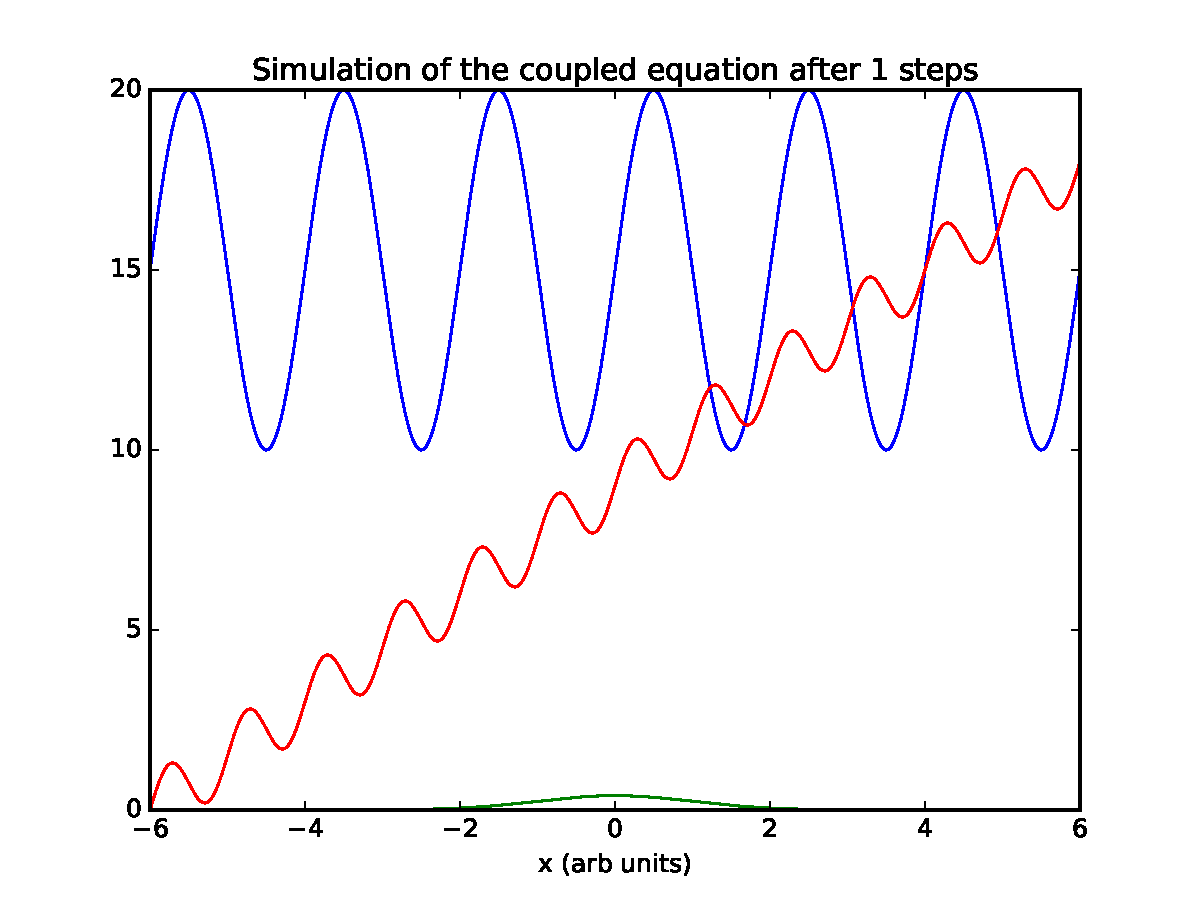
\includegraphics[width=0.45\columnwidth]{CoupledEquationFiniteDifferencesInitial}
	}
\quad
	\subfigure{
		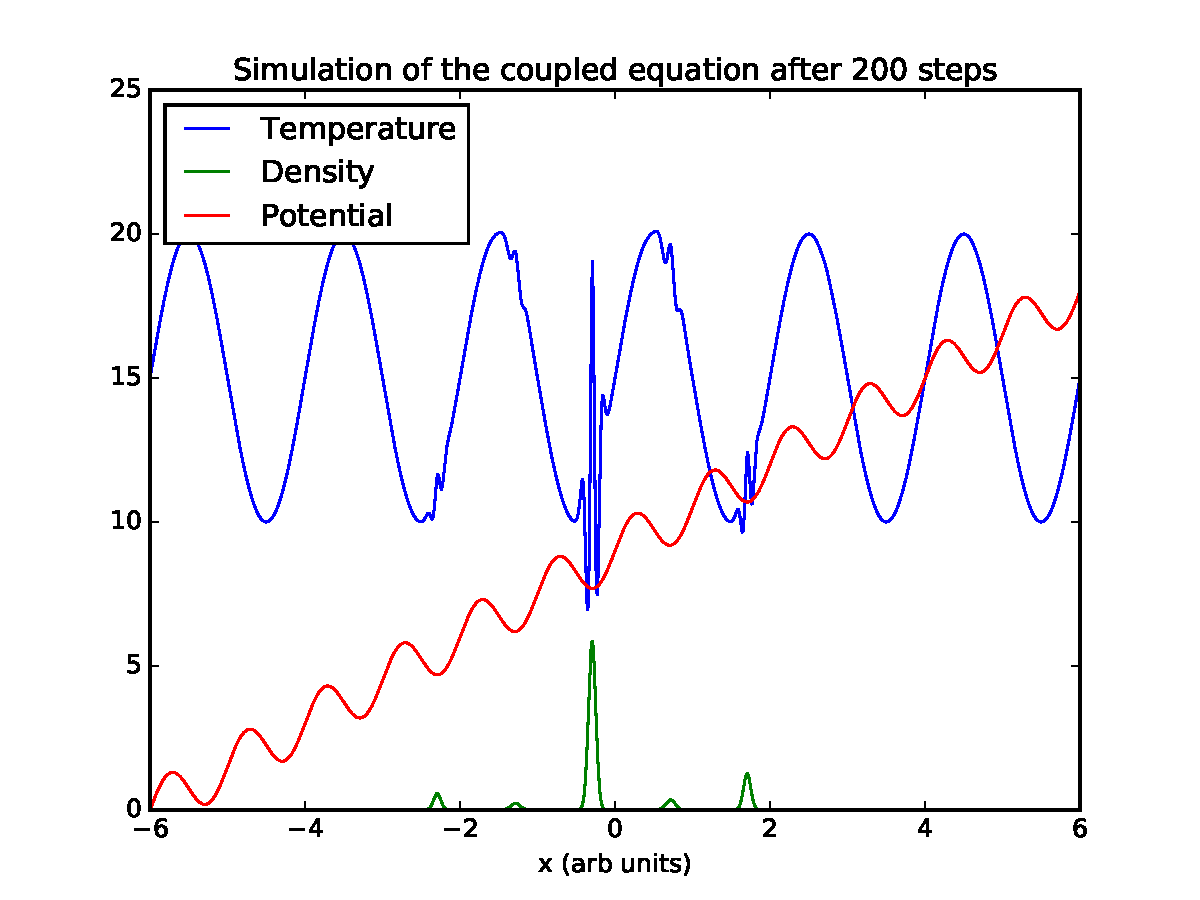
\includegraphics[width=0.45\columnwidth]{CoupledEquationFiniteDifferences}
	}
\caption{Finite differencing simulation of a distribution of particles, we see that the particles are locally interacting with the environment thermally.}
\label{fig:FiniteDifferences}
\end{figure}

\begin{figure}[tb]
	\centering
	\subfigure{%
		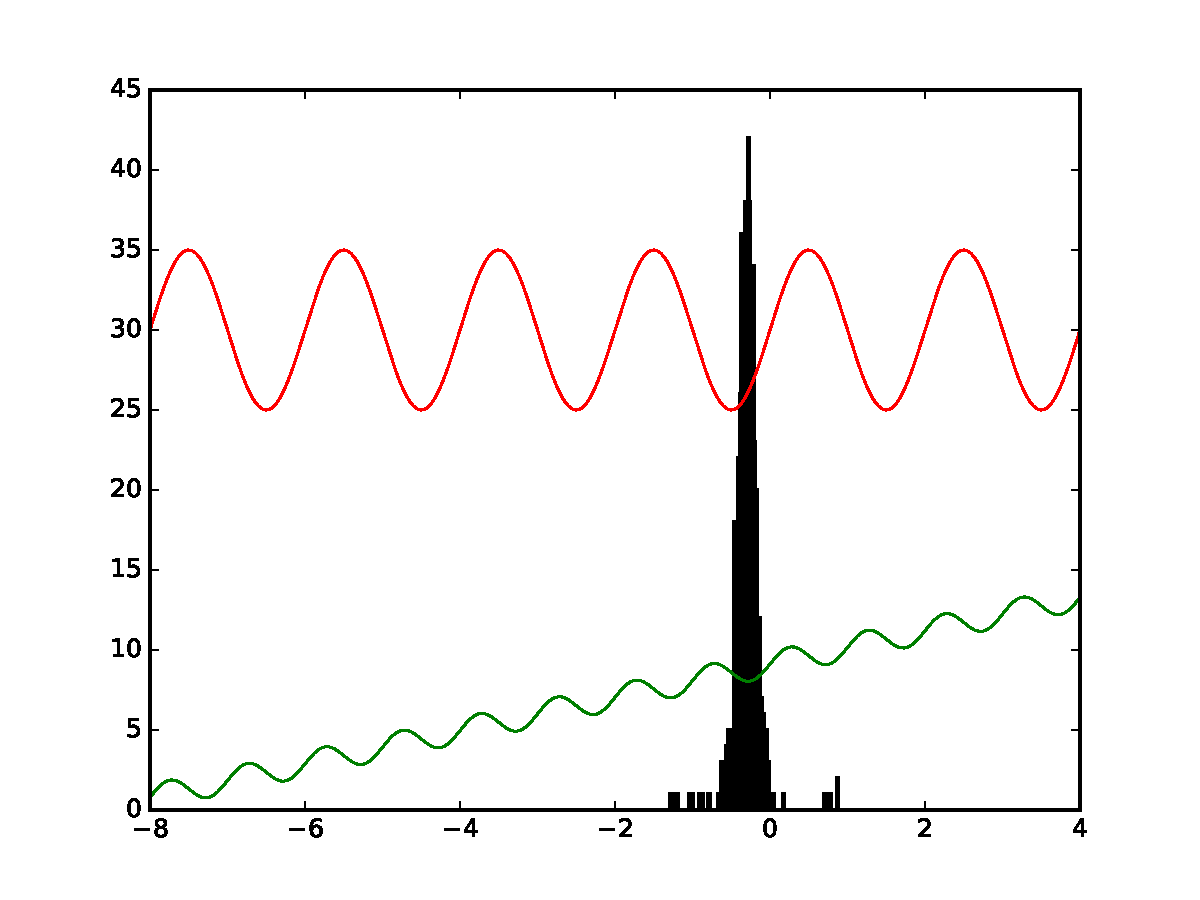
\includegraphics[width=0.45\columnwidth]{CoupledEquationStochasticInitial}
	}
\quad
	\subfigure{
		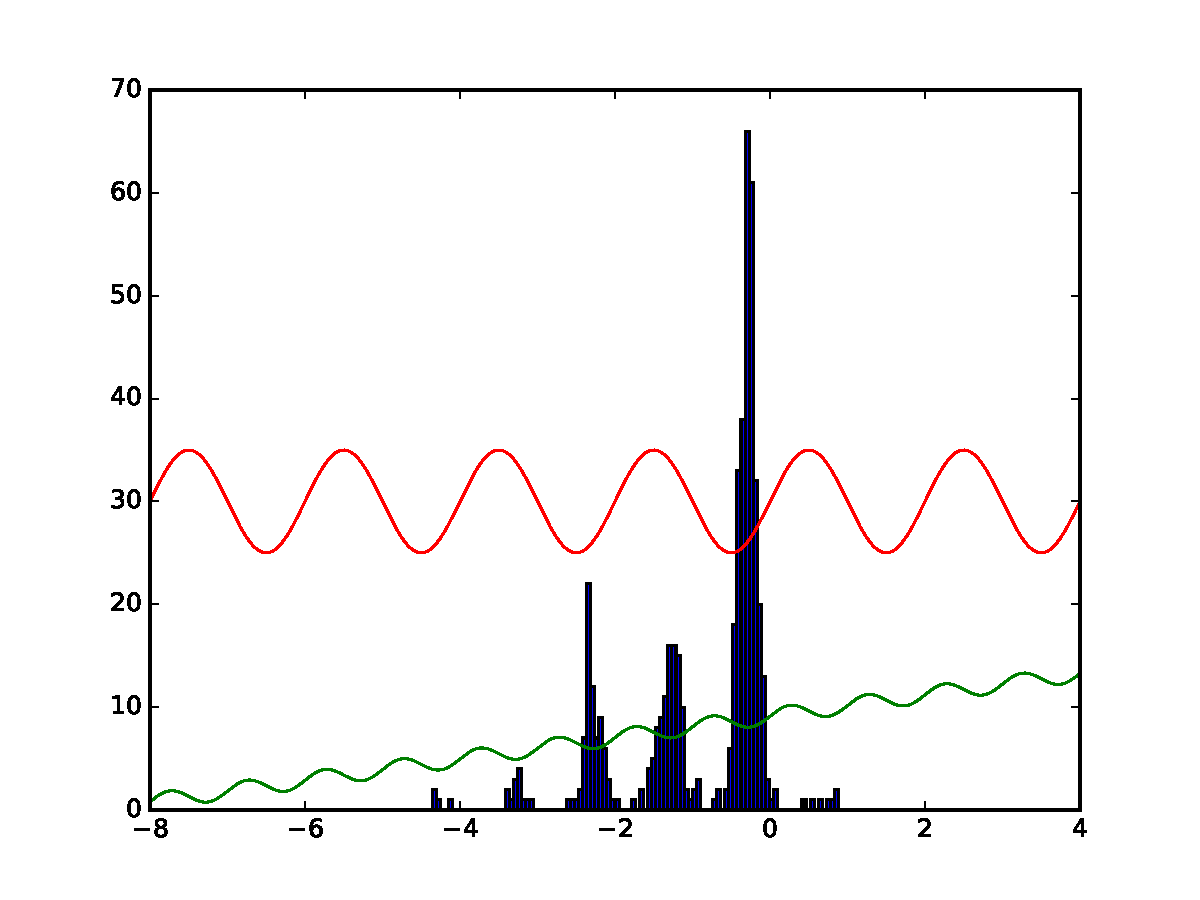
\includegraphics[width=0.45\columnwidth]{CoupledEquationStochastic}
	}
\caption{Stochastic simulation of a distribution of particles, In this simulation we have coupled the equations so that the diffusion of the particles is dependent on the temperature, however the temperature is not affected by the particles (i.e. in the case where $\kappa \to 0$).}
\label{fig:Stochastic}
\end{figure}

Meanwhile, figure \ref{fig:Stochastic} shows a similar situation that has been simulated stochastically. In this case, we  are able to deal with a temperature that is non constant in space, however we are not able to quantify the particles interaction with the environment. This means that $\kappa$ vanishes in our stochastic model. In the future, we aim to be able to deal with these thermal interactions by using the microscopic equations given by Streater \cite{Streater1997, Streater1997a}.


%------------------------------------------------

%------------------------------------------------

%----------------------------------------------------------------------------------------
%	BIBLIOGRAPHY
%----------------------------------------------------------------------------------------

%\renewcommand{\refname}{\spacedlowsmallcaps{References}} % For modifying the bibliography heading

\clearpage{}   % Make sure that the references are on a new page.
\bibliography{BibData}{} % The file containing the bibliography

\bibliographystyle{unsrt}
%----------------------------------------------------------------------------------------

\end{document}
